% !TEX root = ../../main.tex
\chapter{QCD Estimation}
\label{ch:qcd}

Although the lepton isolation and identification working points (\Ch{\ref{ch:objreco}}) have large rejection ratios, the QCD multijet cross section is very large, and may contaminate the control regions and signal regions after reconstruction as fake leptons. The most common sources of fake electrons are from heavy quark decays, photon conversions, and hadrons faking electrons. Non-prompt muons from decays of $b$ and $c$ hadrons are the main source of fake muons. 

The multijet background is steeply falling with \MET. As a first step at rejecting this reducible background, a cut requiring $\MET>100\,\GeV$ is required. During a previous iteration of this search, corresponding to an integrated luminosity of 13.2\,\ifb, the ICHEP analysis~\cite{ichep2016supportnote} determined this cut was sufficient to eliminate the multijet contamination to less than $1\,\%$.  However, the electron channel ($e$-channel) exhibited a discrepancy between data and MC for electrons with high-\pT in the \Wjets control region (CR). This effect was not observed in the muon channel ($\mu$-channel). To account for the discrepancy, a systematic uncertainty on the \Wjets background was added.

Following the ICHEP analysis, an investigation into the discrepancy was performed. It was found that high-\pT events in the $e$-channel with correspondingly small \MET (with respect to the $\pT(e)$) where most likely the result of multijet events faking an electron. The relatively low stats in the high-\pT region amplified the effect of the previously estimated small QCD contamination. In \Sect{\ref{ch:qcd:mjcut}}, a discussion of the implemented multijet cut, to address these high-$\pT(e)$ events is presented. After implementing the multijet cut, a data driven QCD estimation is again performed in~\Sect{\ref{ch:qcd:est}}.

%
\section{Multijet Cut}
\label{ch:qcd:mjcut}
The discrepancy observed in the \Wjets CR for high-$\pT$ electrons was thought to come from multijet events. Since multijet events characteristically have low \MET, the ratio of $\MET/\pT(W\ra e\nu)$ should be relatively low for multijets faking high-\pT electrons. \Fig{\ref{fig:qcd_reg}} shows $\MET/\pT(W\ra e\nu)$ in the \Wjets CR with inverted and relaxed \MET cuts.  
\begin{figure}[h!tb]
\centering
\subfloat[]{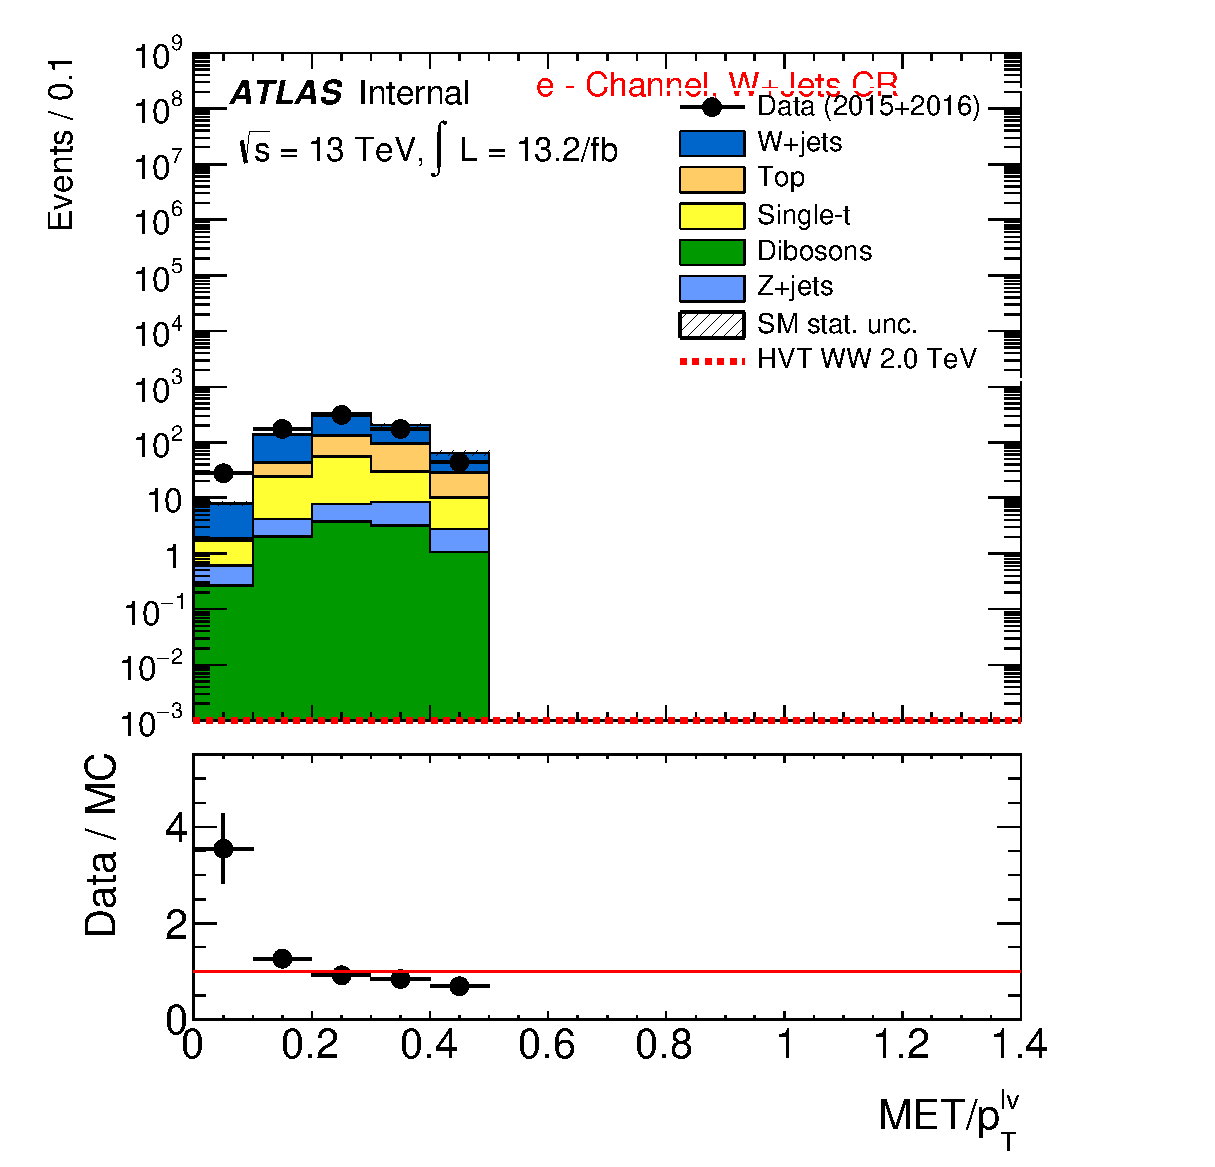
\includegraphics[width=.46\textwidth]{figures/Appendix/qcd/jetjet/InvMET_HP_WCR_e}\label{fig:qcd_reg:a}}
\subfloat[]{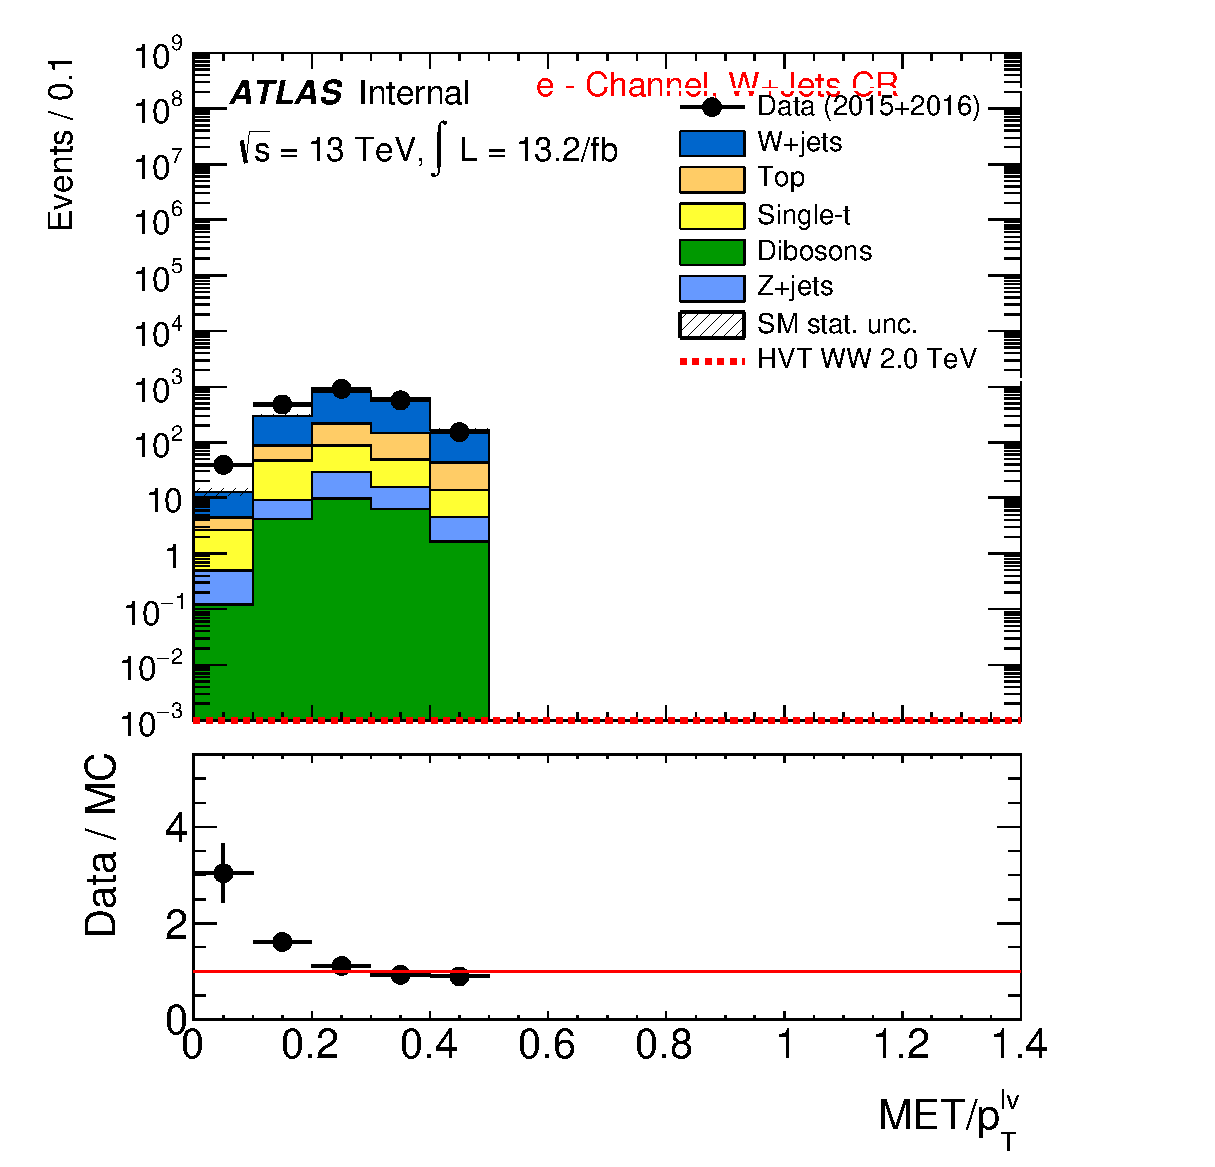
\includegraphics[width=.46\textwidth]{figures/Appendix/qcd/jetjet/InvMET_LP_WCR_e}\label{fig:qcd_reg:b}}\\
\subfloat[]{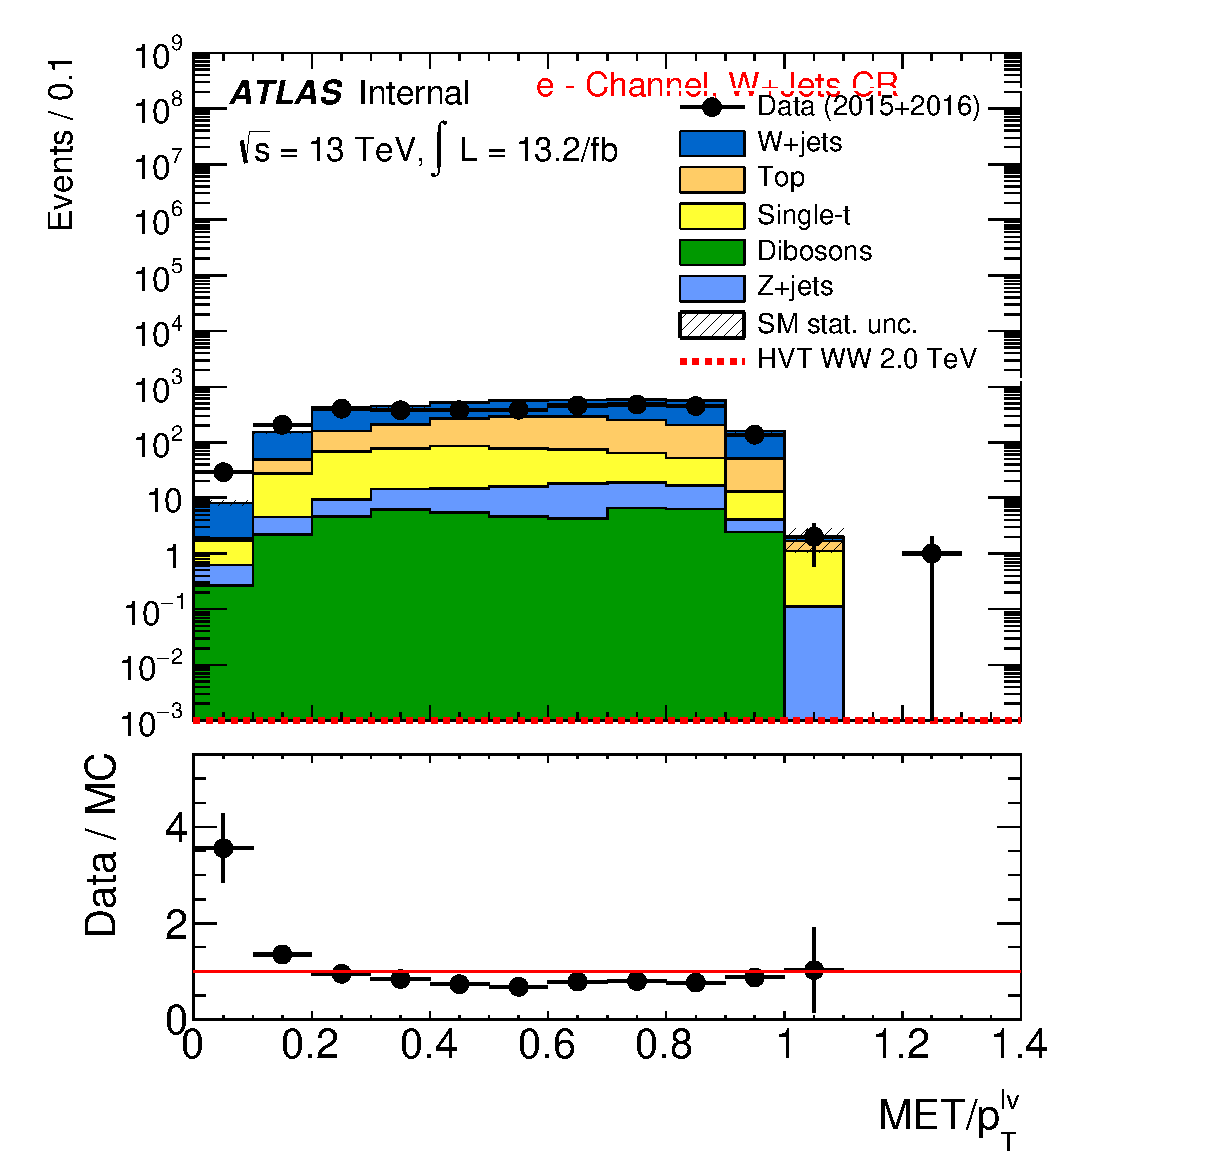
\includegraphics[width=.46\textwidth]{figures/Appendix/qcd/jetjet/RelaxedMET_HP_WCR_e}\label{fig:qcd_reg:c}}
\subfloat[]{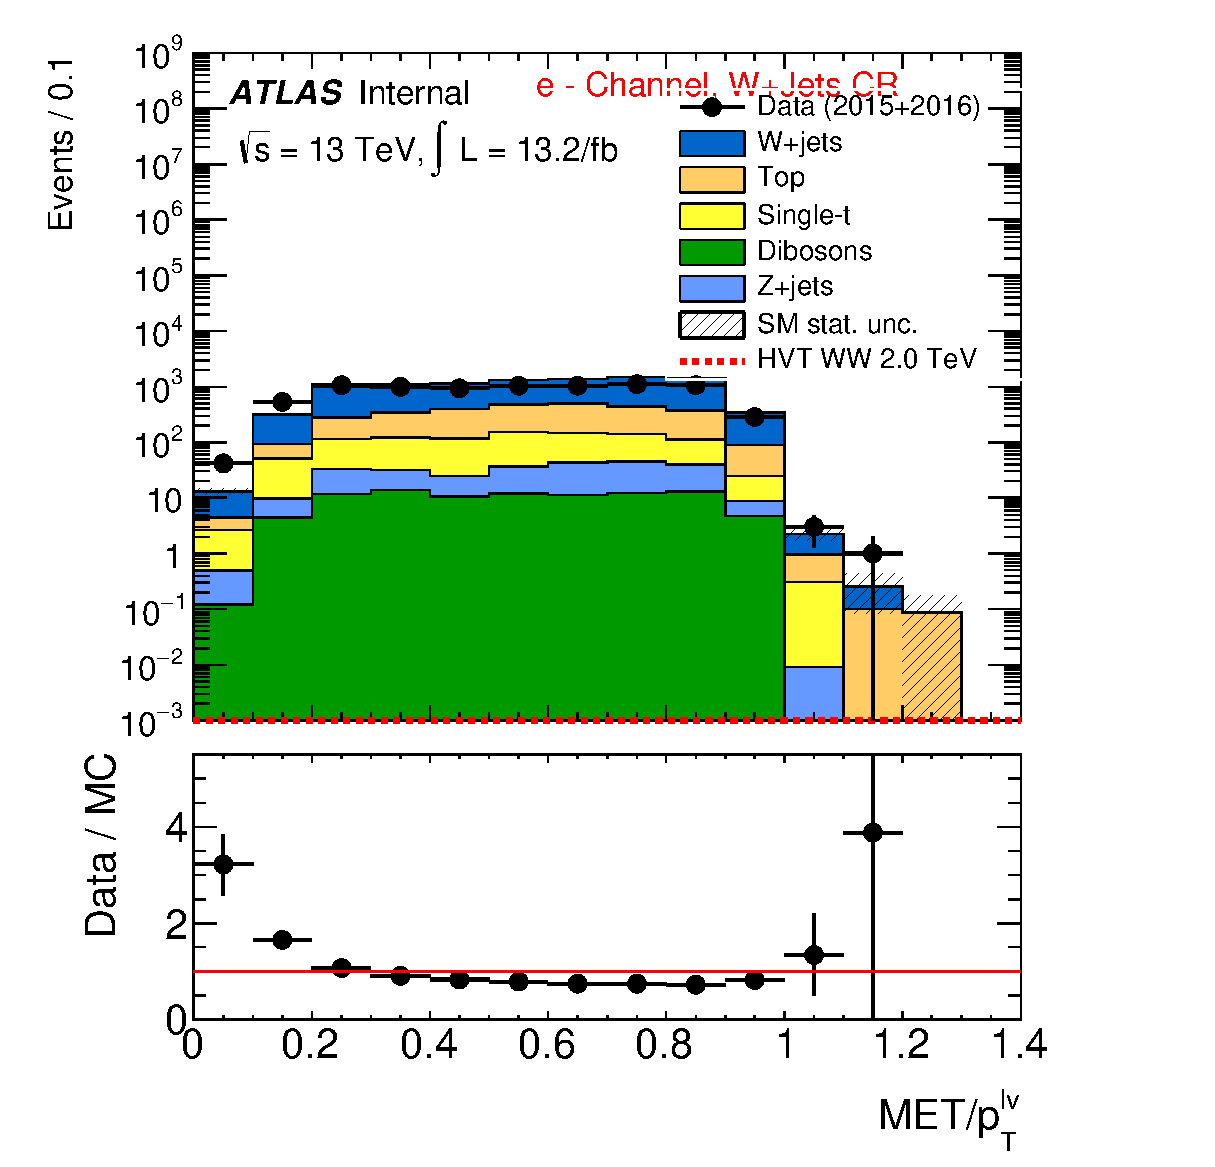
\includegraphics[width=.46\textwidth]{figures/Appendix/qcd/jetjet/RelaxedMET_LP_WCR_e}\label{fig:qcd_reg:d}}
\caption[Distribution of $\MET/\pT(W\ra e\nu)$ in the \Wjets control region with inverted and relaxed \MET cuts. ]{Distribution of $\MET/\pT(W\ra e\nu)$ in the \Wjets CR with inverted \MET selection for \protect\subref{fig:qcd_reg:a} high purity (HP) and  \protect\subref{fig:qcd_reg:b} low purity (LP). The same distribution in the \Wjets CR with relaxed \MET selection for \protect\subref{fig:qcd_reg:c} HP and \protect\subref{fig:qcd_reg:d} LP. }
\label{fig:qcd_reg}
\end{figure}

\clearpage
The inverted \MET selection represents an enriched QCD region. The mis-modeling between data and MC is largest for small values of $\MET/\pT(W\ra e\nu)$ as expected. The relaxed \MET selection shows mis-modeling in the same region as the multijet enriched selection. A di-jet MC sample generated with \textsc{Pythia8} was used as a cross check. In~\Fig{\ref{fig:qcdpt_el}}, the di-jet MC confirms the concentration of QCD contamination in the high-$\pT(e)$ region.
\begin{figure}[h!tb]
\centering
\subfloat[]{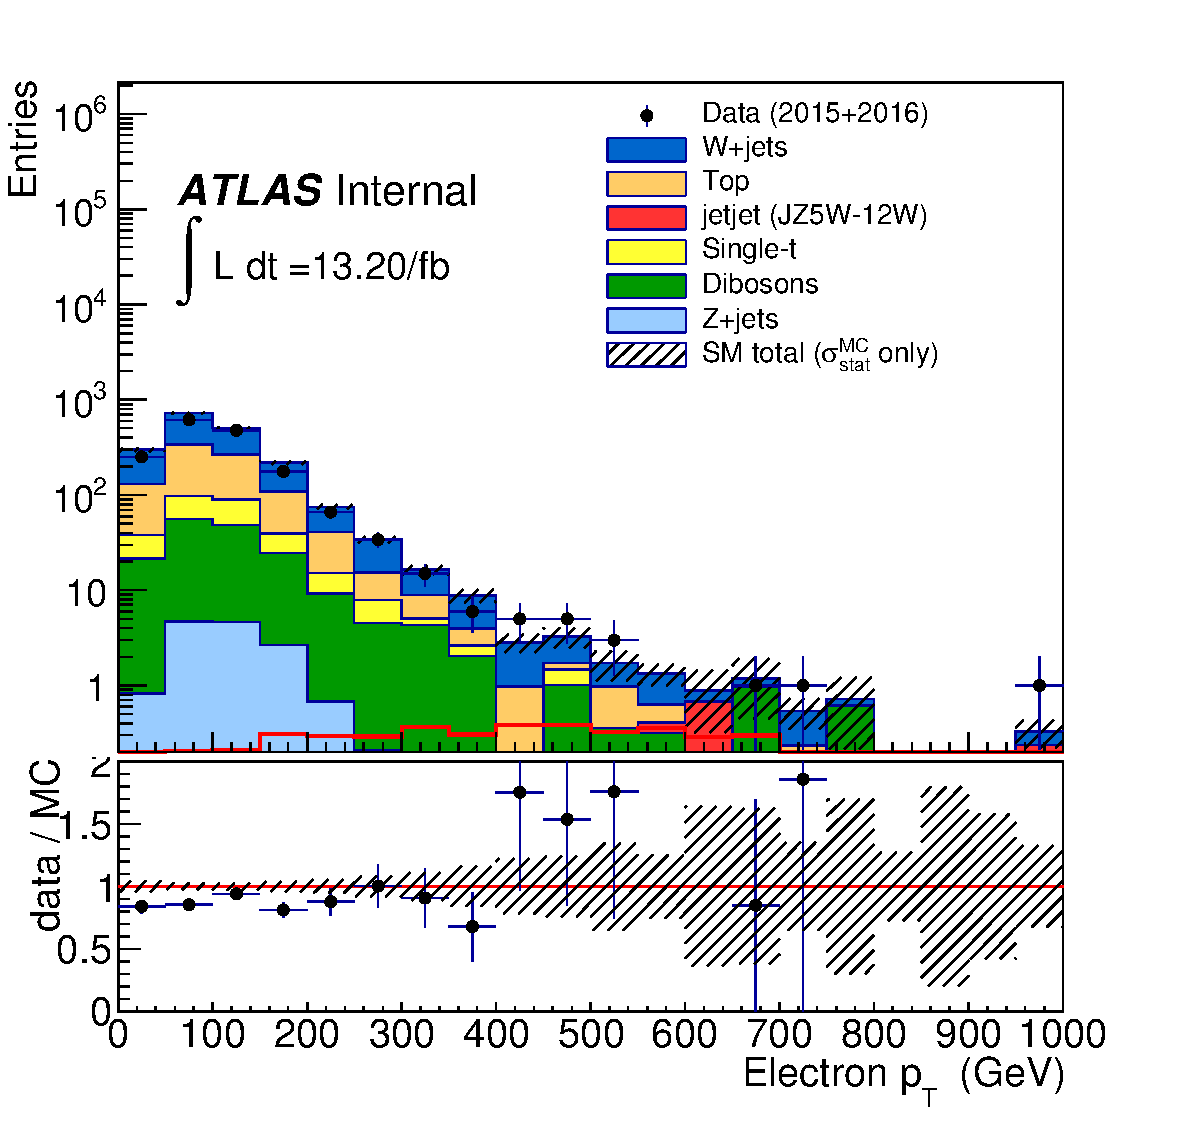
\includegraphics[width=.48\textwidth]{figures/Appendix/qcd/elPt_SRWWHP}\label{fig:qcdpt_el:a}}
\subfloat[]{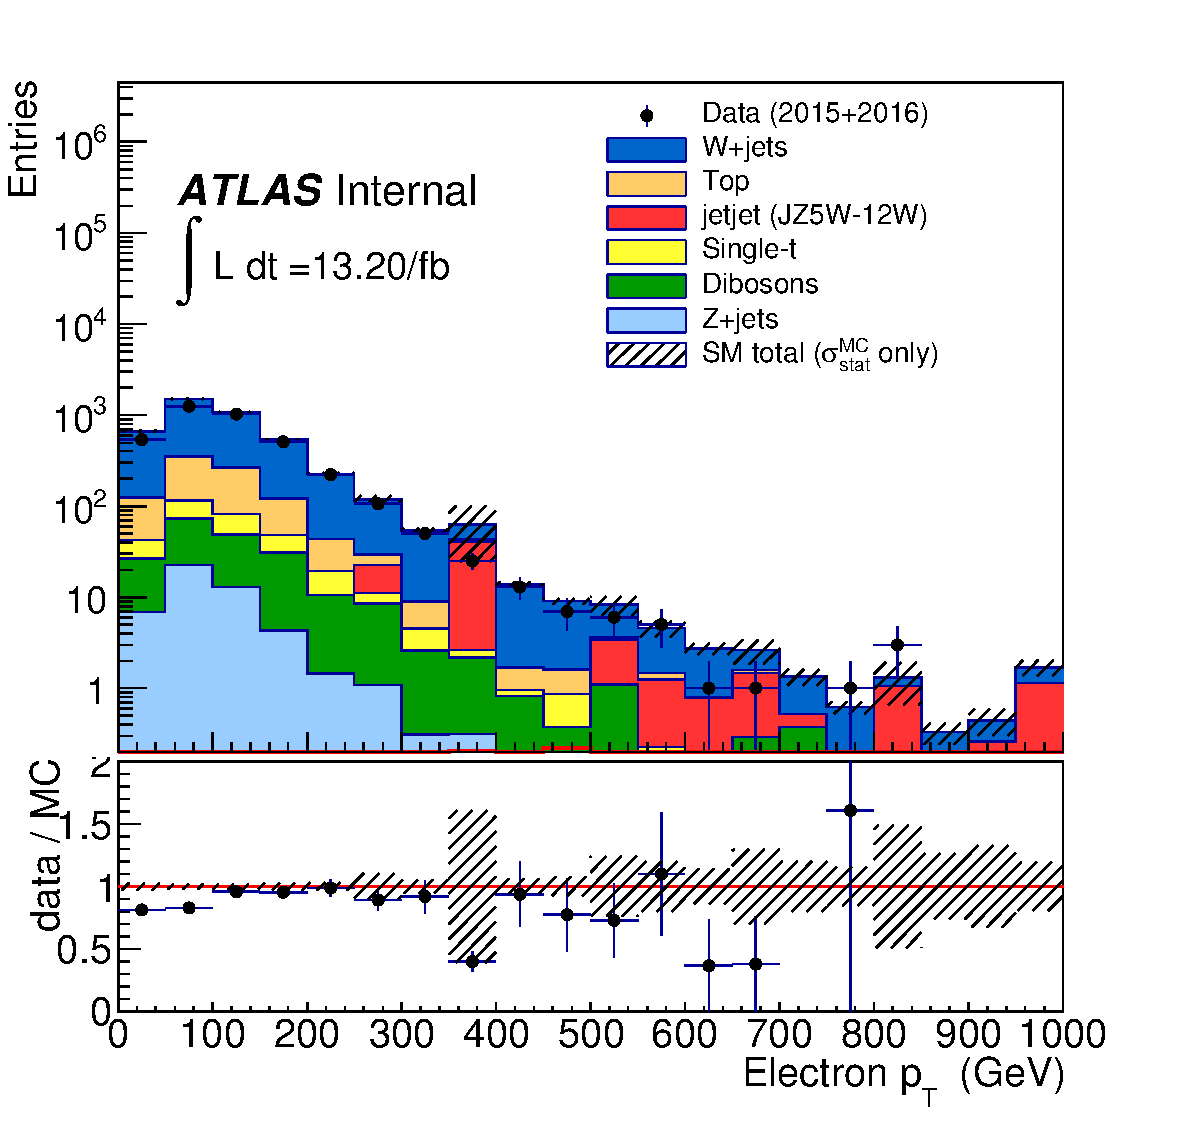
\includegraphics[width=.48\textwidth]{figures/Appendix/qcd/elPt_SRWWLP}\label{fig:qcdpt_el:b}}\\
\subfloat[]{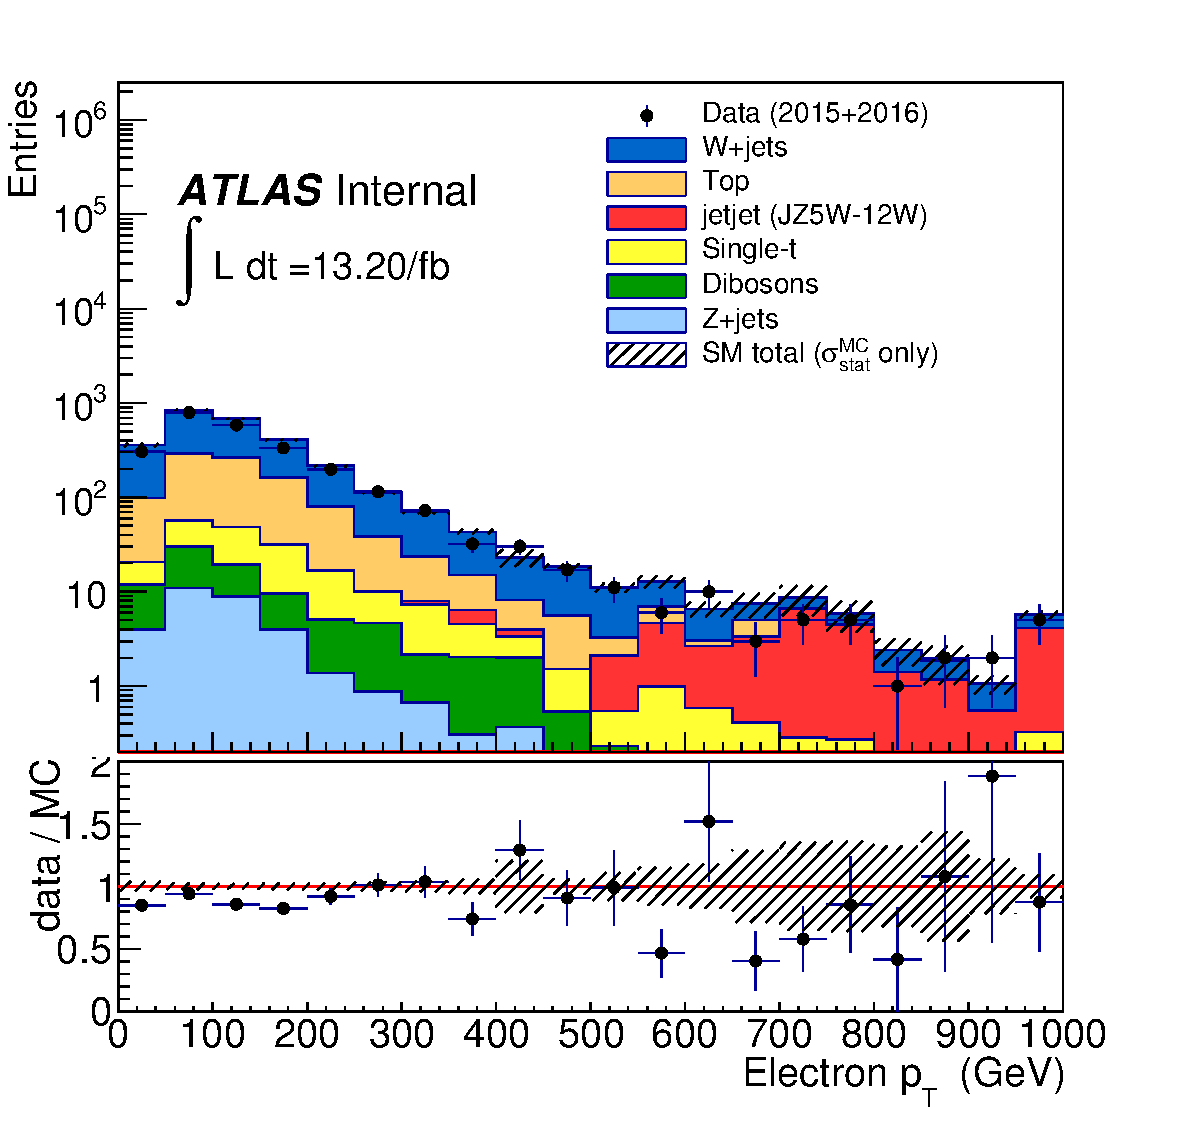
\includegraphics[width=.48\textwidth]{figures/Appendix/qcd/elPt_CRWHP}\label{fig:qcdpt_el:c}}
\subfloat[]{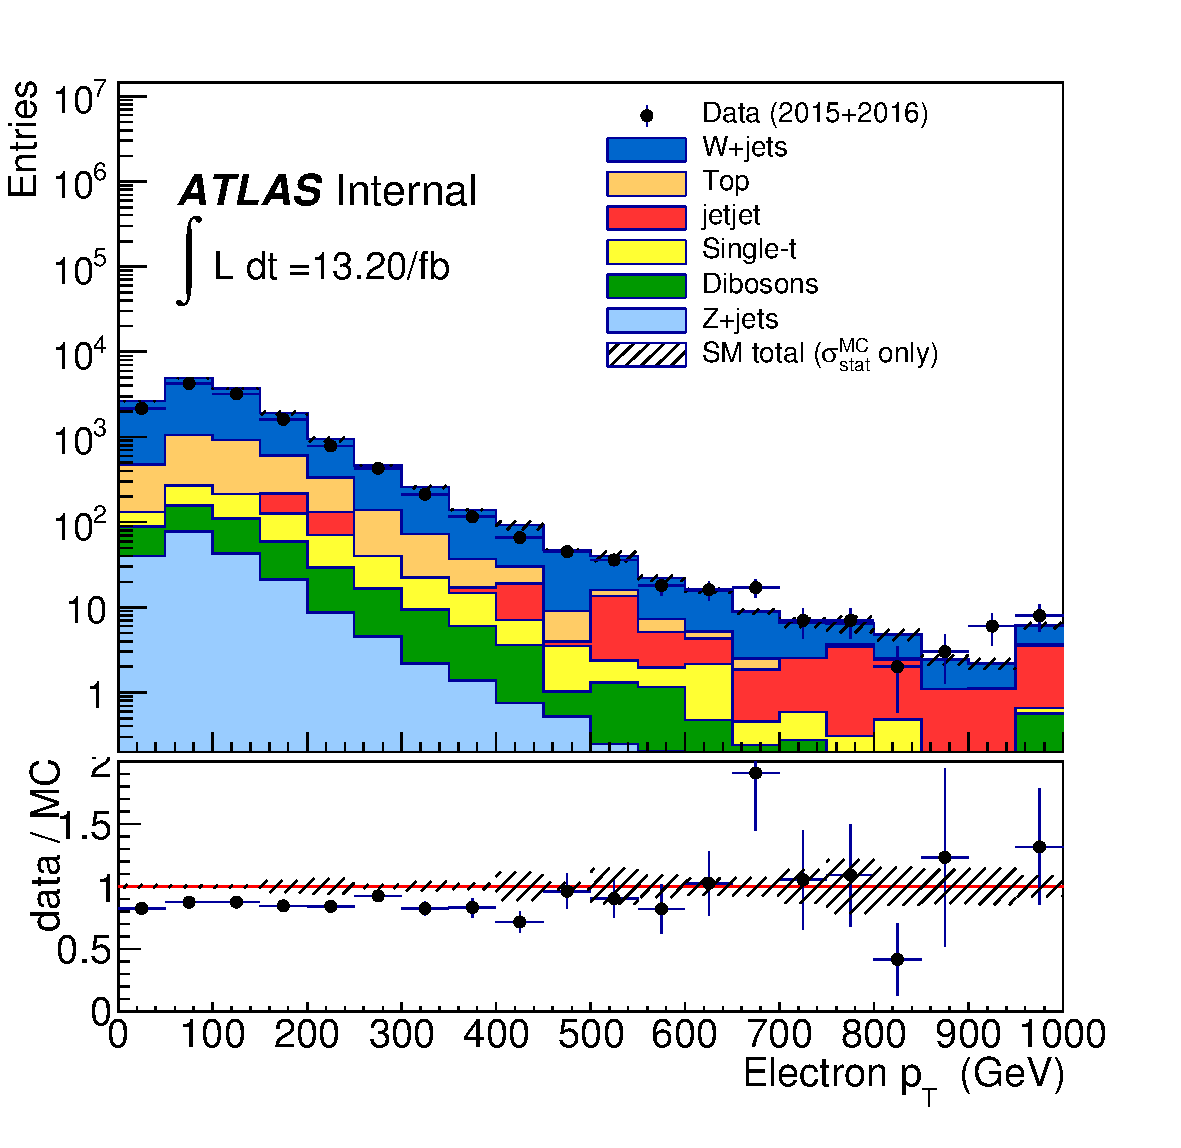
\includegraphics[width=.48\textwidth]{figures/Appendix/qcd/elPt_CRWLP}\label{fig:qcdpt_el:d}}
\caption[Electron $\pT$ distribution including a di-jet Monte Carlo sample]{Distribution of $\pT(e)$ for \protect\subref{fig:qcdpt_el:a} high purity (HP) SR, \protect\subref{fig:qcdpt_el:b} low purity (LP) SR, \protect\subref{fig:qcdpt_el:c} HP \Wjets CR, and \protect\subref{fig:qcdpt_el:d} LP \Wjets CR. The \textsc{Pythia8} di-jet MC samples verify concentration of multijet contamination in the high-\pT region.}
\label{fig:qcdpt_el}
\end{figure}

\clearpage
In~\Fig{\ref{fig:metpt_el}}, the di-jet MC indicates the multijet contribution is largely concentrated in the region $\MET/\pT(W\ra e\nu)<0.2$ for the $e$-channel, as hinted by~\Fig{\ref{fig:qcd_reg}}. \Fig{\ref{fig:metpt_mu}} confirms the negligible contamination in the $\mu$-channel.  
\begin{figure}[htb]
\centering
\subfloat[]{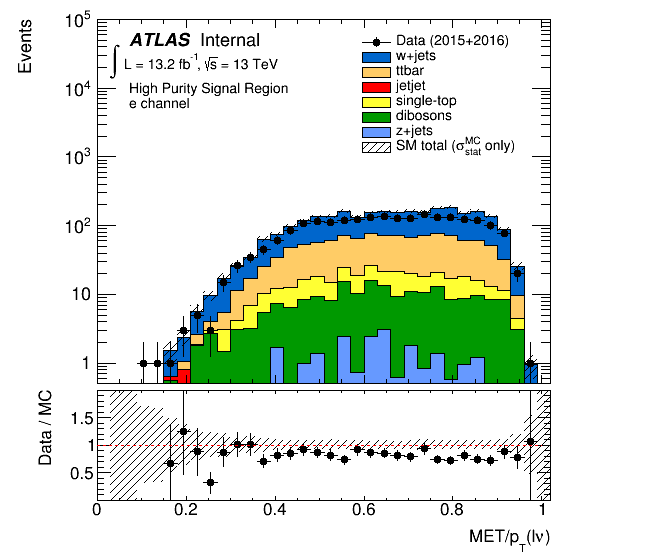
\includegraphics[width=.48\textwidth]{figures/Appendix/qcd/jetjet/metpt_0_el}\label{fig:metpt_el:a}}
\subfloat[]{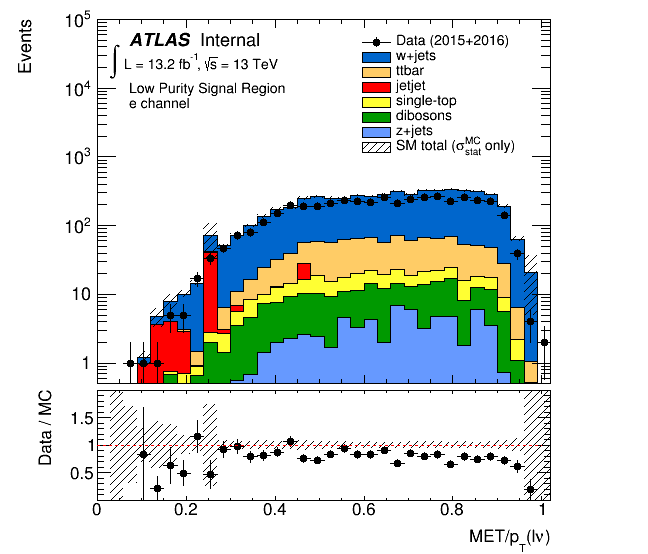
\includegraphics[width=.48\textwidth]{figures/Appendix/qcd/jetjet/metpt_11_el}\label{fig:metpt_el:b}}\\
\subfloat[]{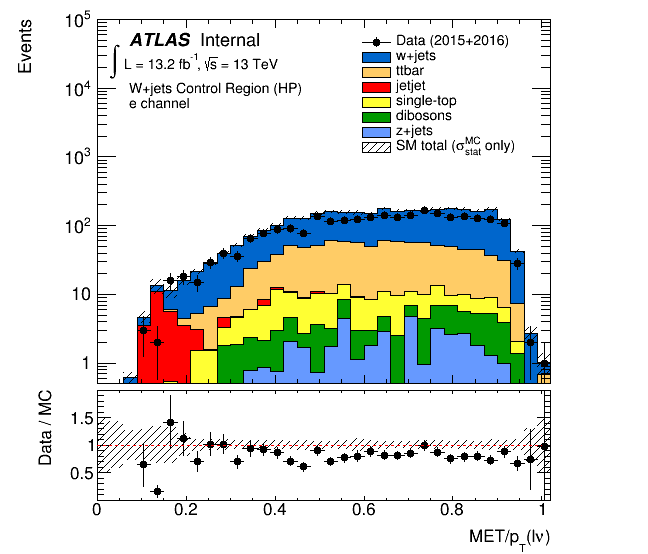
\includegraphics[width=.48\textwidth]{figures/Appendix/qcd/jetjet/metpt_3_el}\label{fig:metpt_el:c}}
\subfloat[]{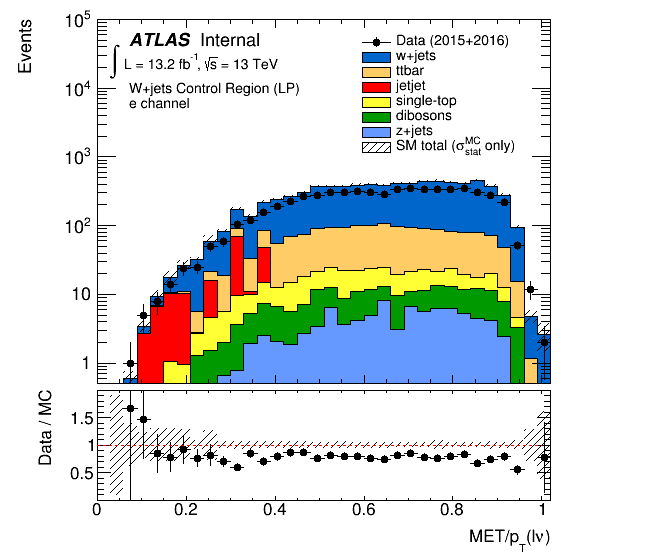
\includegraphics[width=.48\textwidth]{figures/Appendix/qcd/jetjet/metpt_12_el}\label{fig:metpt_el:d}}
\caption[Distribution of $\MET/\pT(W\ra e\nu)$ including a di-jet Monte Carlo sample]{Distribution of $\MET/\pT(W\ra\ell\nu)$ for the $e$-channel in \protect\subref{fig:metpt_el:a} high purity (HP) SR, \protect\subref{fig:metpt_el:b} low purity (LP) SR, \protect\subref{fig:metpt_el:c} HP \Wjets CR, and \protect\subref{fig:metpt_el:d} LP \Wjets CR. The \textsc{Pythia8} di-jet MC samples verify the multijet contamination is mostly concentrated in the region $\MET/\pT(W\ra e\nu)$. }
\label{fig:metpt_el}
\end{figure}
\begin{figure}[h!tb]
\centering
\subfloat[]{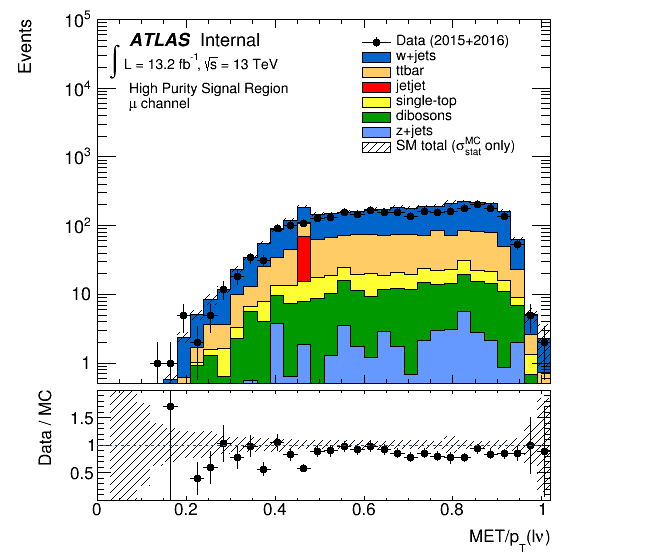
\includegraphics[width=.48\textwidth]{figures/Appendix/qcd/jetjet/metpt_0_mu}\label{fig:metpt_mu:a}}
\subfloat[]{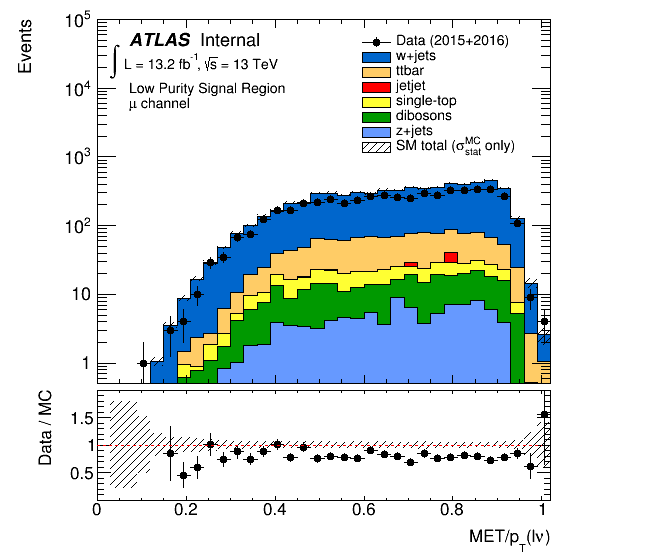
\includegraphics[width=.48\textwidth]{figures/Appendix/qcd/jetjet/metpt_11_mu}\label{fig:metpt_mu:b}}\\
\subfloat[]{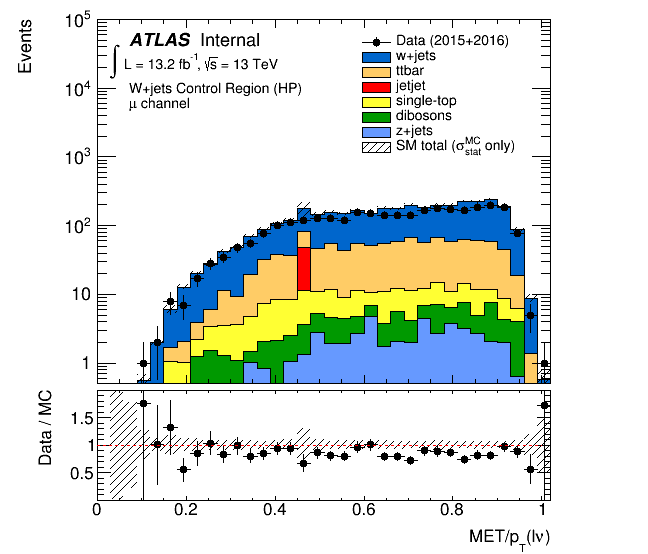
\includegraphics[width=.48\textwidth]{figures/Appendix/qcd/jetjet/metpt_3_mu}\label{fig:metpt_mu:c}}
\subfloat[]{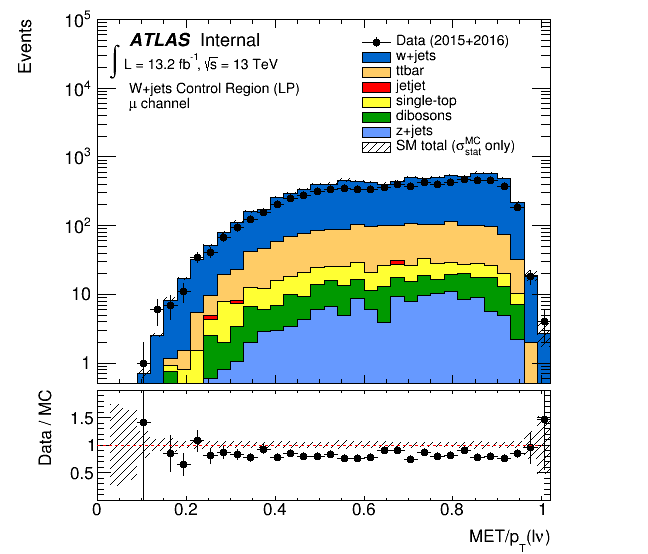
\includegraphics[width=.48\textwidth]{figures/Appendix/qcd/jetjet/metpt_12_mu}\label{fig:metpt_mu:d}}
\caption[Distribution of $\MET/\pT(W\ra \mu \nu)$ including a di-jet Monte Carlo sample]{Distribution of $\MET/\pT(W\ra\ell\nu)$ for the $\mu$-channel in \protect\subref{fig:metpt_mu:a} high purity (HP) SR, \protect\subref{fig:metpt_mu:b} low purity (LP) SR, \protect\subref{fig:metpt_mu:c} HP \Wjets CR, and \protect\subref{fig:metpt_mu:d} LP \Wjets CR. The \textsc{Pythia8} di-jet MC samples verify negligible contamination in the $\mu$-channel.}
\label{fig:metpt_mu}
\end{figure}

% Signal efficiency
\clearpage
To remove this contamination, a multijet cut is proposed by requiring $\MET/\pT(W\ra e\nu)>0.2$, for the $e$-channel only. \Fig{\ref{fig:metpt_eff}} shows the efficiency and significance for various minimum cut values of $\MET/\pT(W\ra e\nu)$ for a simulated HVT $W$' ($qq$ fusion production) and heavy Higgs (VBF production) at various resonant masses. The proposed multijet cut has over 90\,\% signal efficiency for all masses.
\begin{figure}[htb]
\centering
\subfloat[]{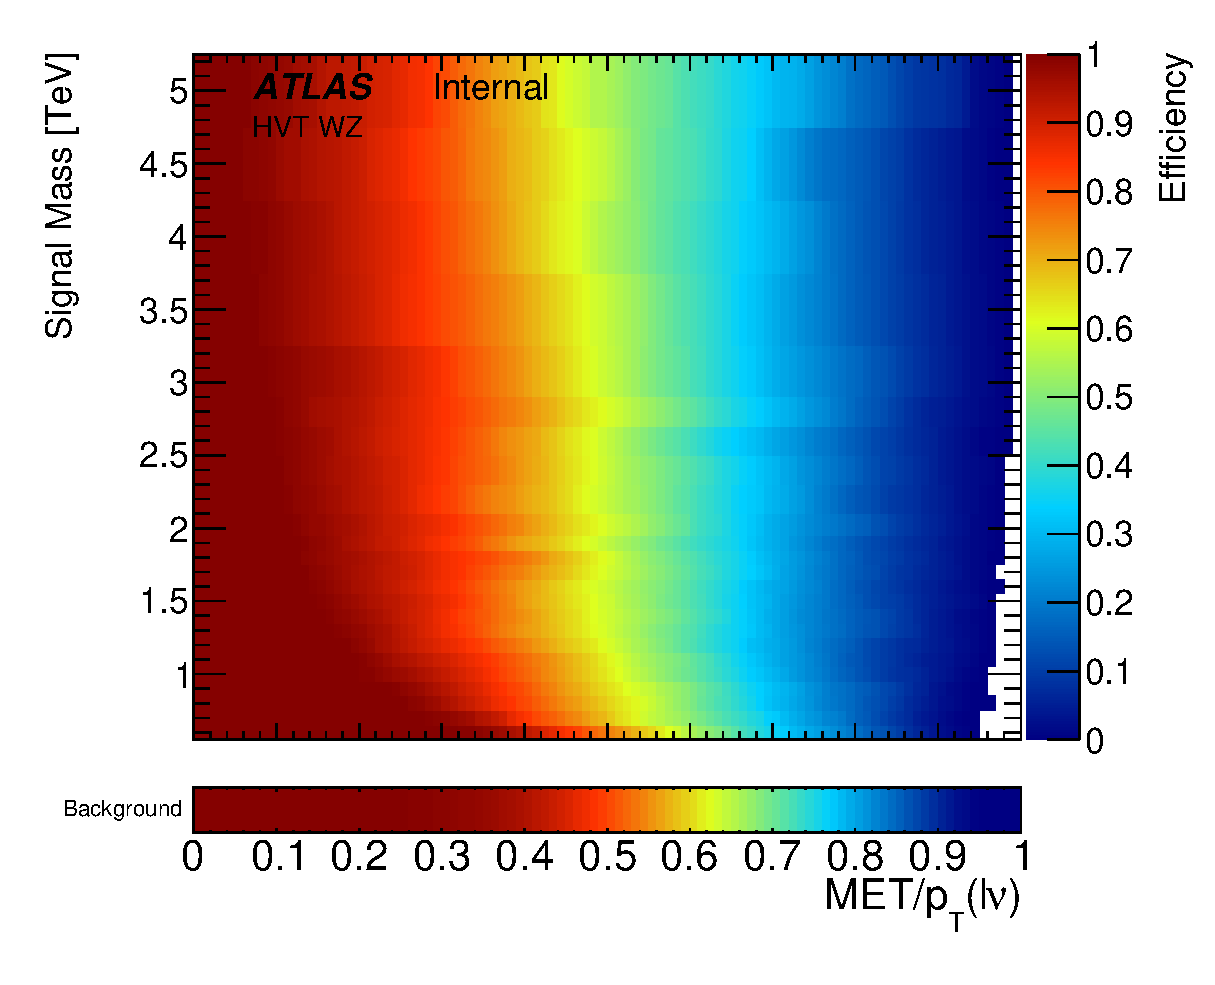
\includegraphics[width=.48\textwidth]{figures/Appendix/qcd/2d_eff_HVTWZ_met_over_ptlv}\label{fig:metpt_eff:a}}
\subfloat[]{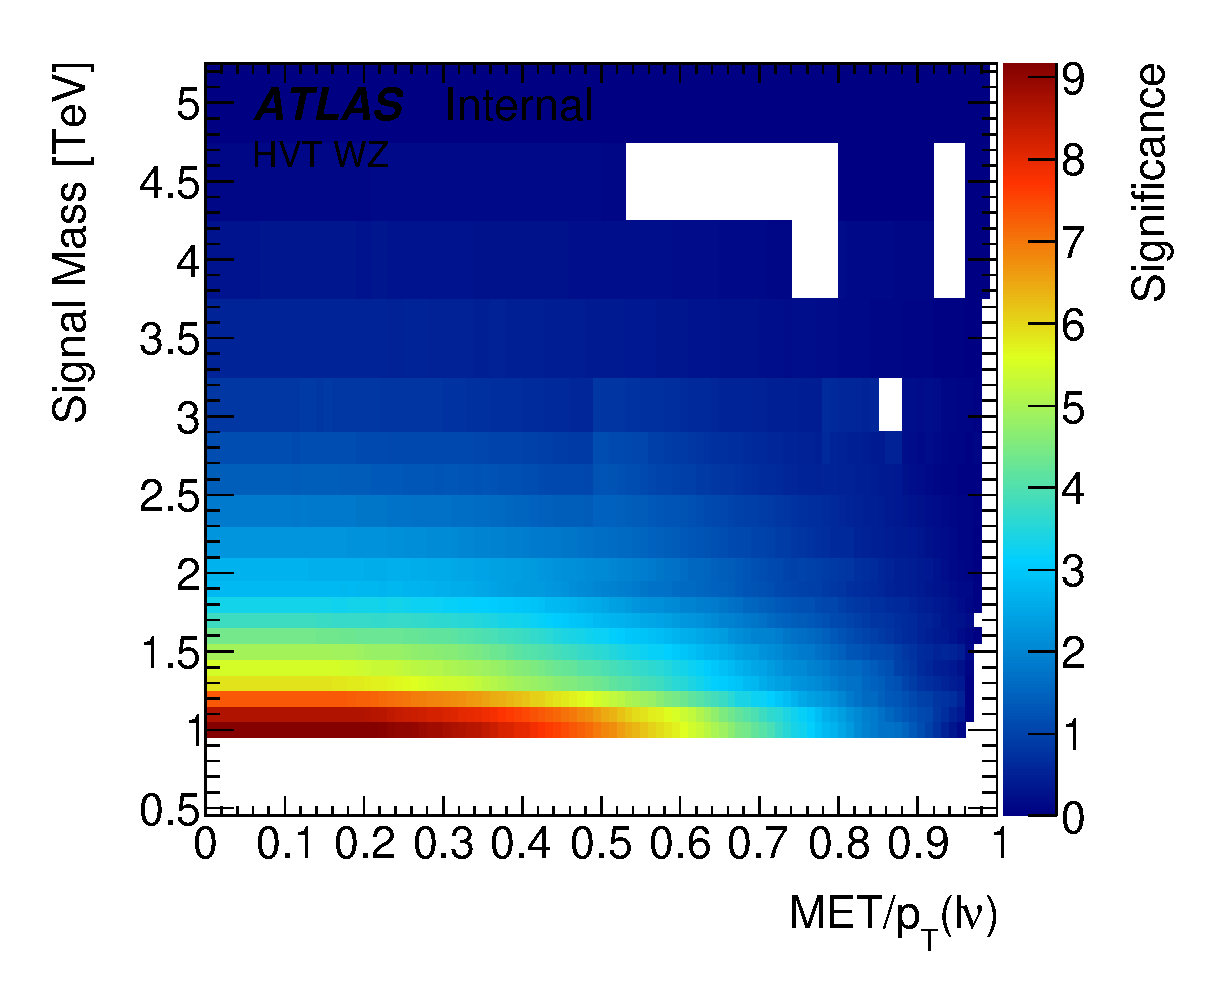
\includegraphics[width=.48\textwidth]{figures/Appendix/qcd/2d_sig_HVTWZ_met_over_ptlv}\label{fig:metpt_eff:b}}\\
\subfloat[]{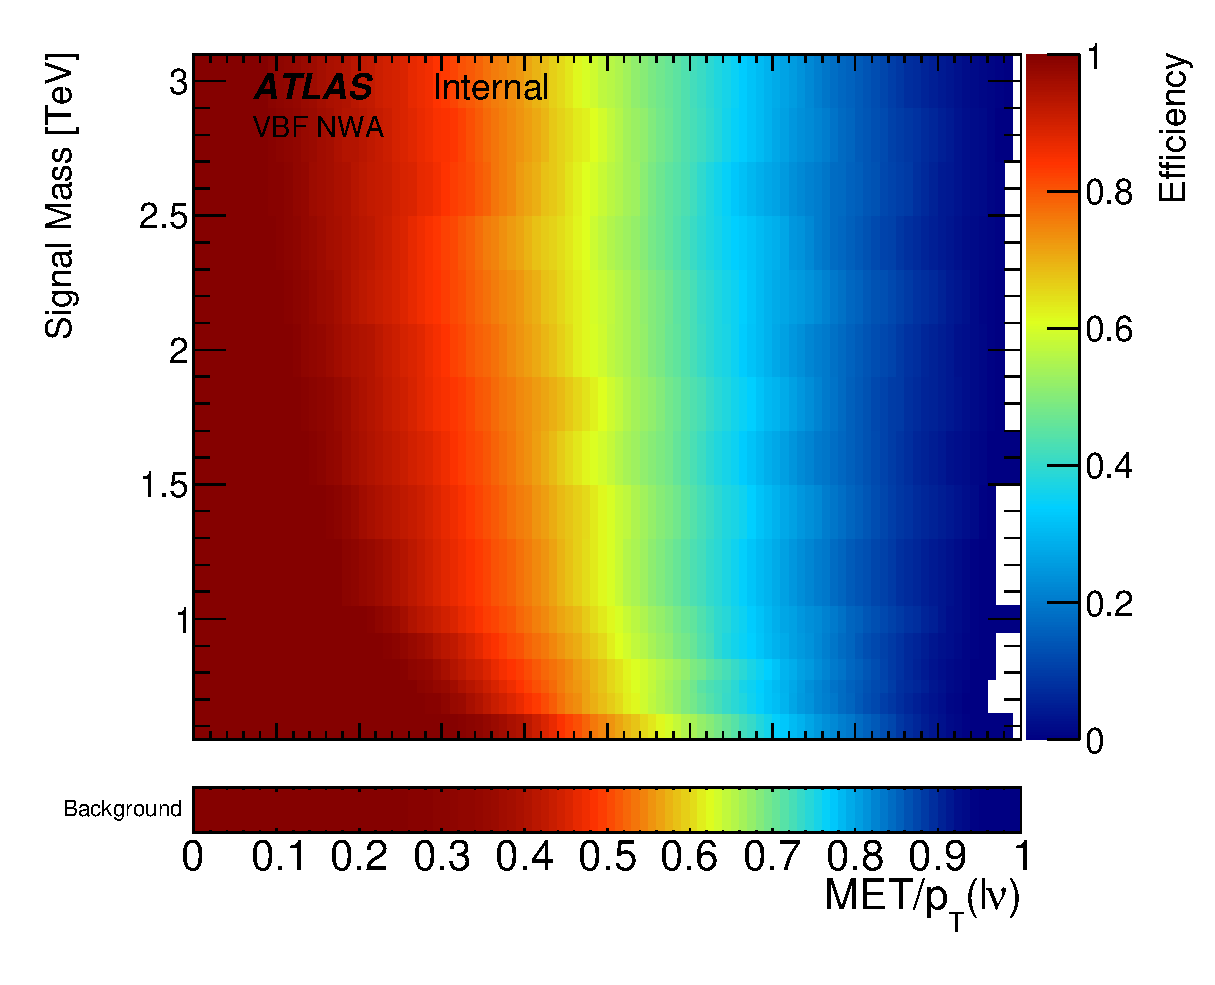
\includegraphics[width=.48\textwidth]{figures/Appendix/qcd/2d_eff_vbfNWA_met_over_ptlv}\label{fig:metpt_eff:c}}
\subfloat[]{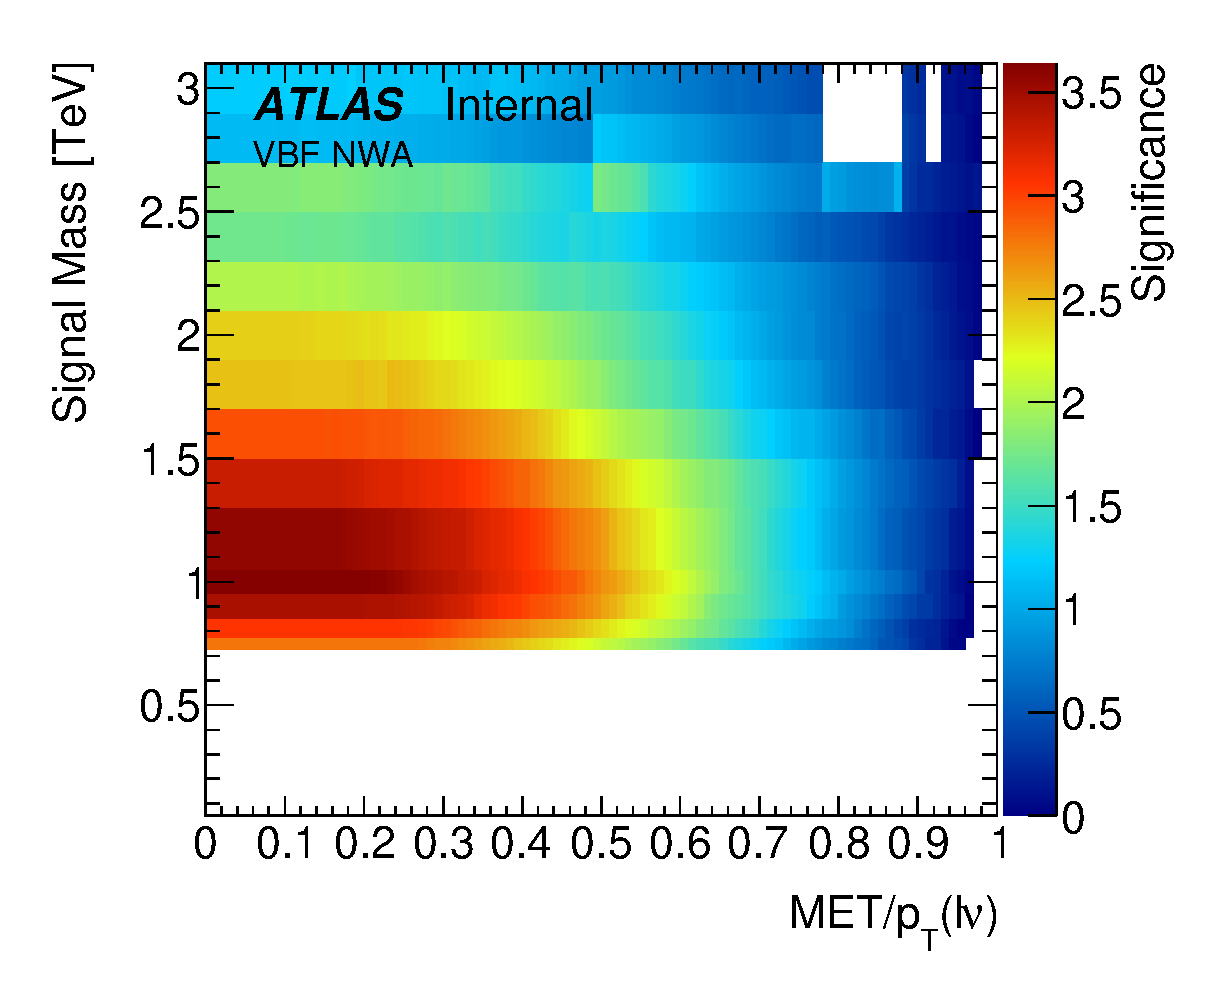
\includegraphics[width=.48\textwidth]{figures/Appendix/qcd/2d_sig_vbfNWA_met_over_ptlv}\label{fig:metpt_eff:d}}
\caption[Signal efficiency and significance of multijet cut for an HVT $W$' and a heavy Higgs]{Using simulated HVT $W$' MC samples for masses from 500\,\GeV\, to 5\,\TeV, the \protect\subref{fig:metpt_eff:a} signal and background efficiency and \protect\subref{fig:metpt_eff:b} expected significance is shown for minimum cut values of $\MET/\pT(W\ra e\nu)$. Simulated heavy Higgs samples with VBF production, for masses from 500\,\GeV\, to 3\,\TeV, are used in \protect\subref{fig:metpt_eff:c} and \protect\subref{fig:metpt_eff:d}. The significance is calculated in a window of $\pm 2\sigma_m$ around the center of the signal mass distribution as $\sigma_{sig}=\sqrt{2\times(s+b)\times\log\left(1+(s/b)\right) - 2s}$.}
\label{fig:metpt_eff}
\end{figure}


%
\clearpage
\section{Data Driven QCD Estimation}
\label{ch:qcd:est}

After implementation of the multijet cut defined in~\Sect{\ref{ch:qcd:mjcut}} to the $e$-channel, a data driven estimation of the QCD contamination is performed with data corresponding to an integrated luminosity of 13.2\,\ifb. A CR is defined, which is expected to be enriched with multijet events, in order to extract a shape template. The multijet shape template is then used to fit the nominal \Wjets CR and estimate the contamination. 

To define the CR for the multijet shape extraction, the lepton identification and isolation requirements are loosened. For the $e$-channel, the electron is required to fail the nominal isolation and LH identification cuts. For the $\mu$-channel, the muon is required to fail the nominal isolation and impact parameter cuts\footnote{
	For the $\mu$-channel, in addition to the nominal \MET triggers used, single muon triggers were added to avoid the trigger turn on for events with low \MET. For 2015 data, the trigger was HLT\_mu20\_iloose\_L1MU15 OR HLT\_mu50. For data from 2016, the trigger was HLT\_mu26\_ivarmedium OR HLT\_mu50. 
}. Both channels are required to pass the ``Loose'' isolation\footnote{
The Loose isolation working point provides variable cuts to ensure 99\,\% efficiency for both calorimeter and track isolation.
} and ``Loose'' identification working points. Events are then required to have exactly one ``loose'' lepton, and no cut on \MET is applied. Then, all events passing the rest of the cuts for either the signal region (SR) or \Wjets CR are considered. The shape is fit separately for high purity (HP) and low purity (LP) regions. 

The non-multijet background is estimated with the same MC samples used in the analysis (\Wjets, \Zjets, \ttbar, \Singlet, and SM diboson samples). In the multijet CR, a multijet shape is extracted by subtracting the MC from the observed data using the \MET distribution. The shape extracted from the multijet CR is used to fit\footnote{
The shape of the MC below 50\,\GeV\, indicates the triggers are still affecting regions of low \MET, so the fit is performed only above 50\,\GeV.
} the \MET distribution in the \Wjets CR (with no \MET cut applied). The normalization of the MC background is allowed to float within statistical uncertainties in the fit. 

The results of the QCD shape extraction and fit for the $e$-channel and $\mu$-channel are shown in~\Fig{\ref{fig:qcdshape_fit_el}} and~\Fig{\ref{fig:qcdshape_fit_mu}}, respectively. For the $e$-channel, the contamination for $\MET>100\,\GeV$ (the selection used in the nominal analysis) is consistent with zero events. The fit for the $e$-channel had a $\chi^2/$ndf value of 1.04 (4.01) for the HP (LP) region. For the $\mu$-channel, the multijet contamination in the multijet CR is already negligible, and the fit region confirms the MC describes the data well.
\begin{figure}[h!bt]
\centering
\subfloat[]{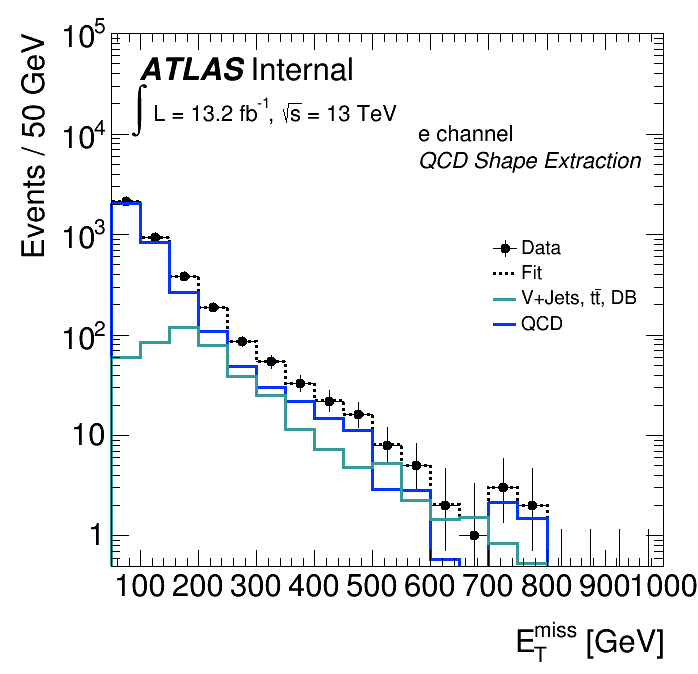
\includegraphics[width=.48\textwidth]{figures/Appendix/qcd/met_qcdshape_el_hp}\label{fig:qcdshape_fit_el:a}}
\subfloat[]{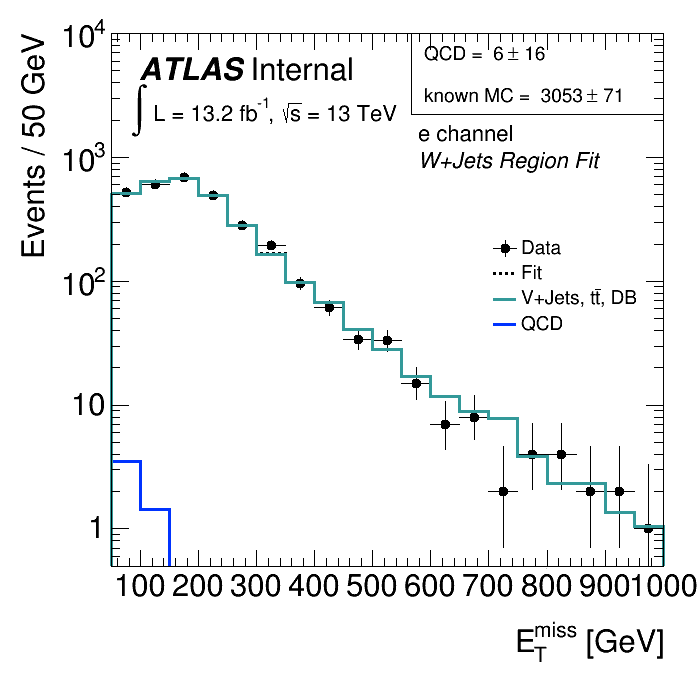
\includegraphics[width=.48\textwidth]{figures/Appendix/qcd/met_wjfit_el_hp}\label{fig:qcdshape_fit_el:b}}\\
\subfloat[]{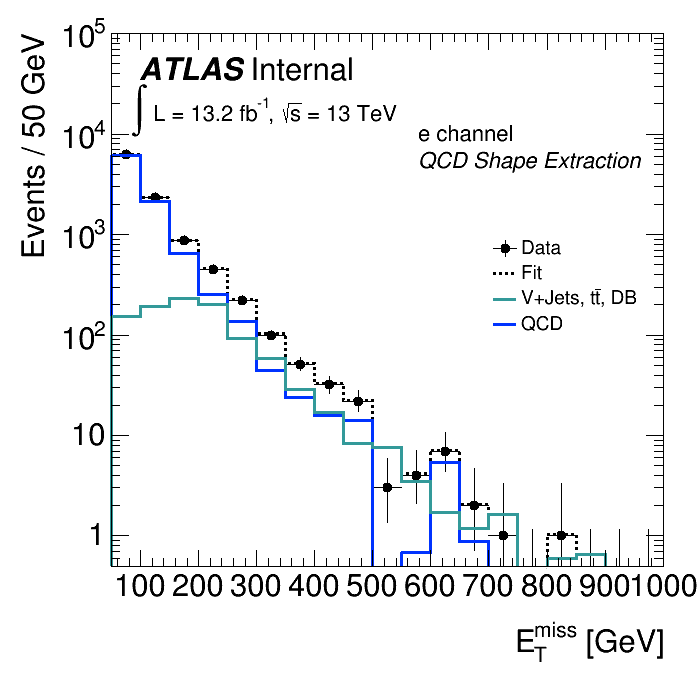
\includegraphics[width=.48\textwidth]{figures/Appendix/qcd/met_qcdshape_el_lp}\label{fig:qcdshape_fit_el:c}}
\subfloat[]{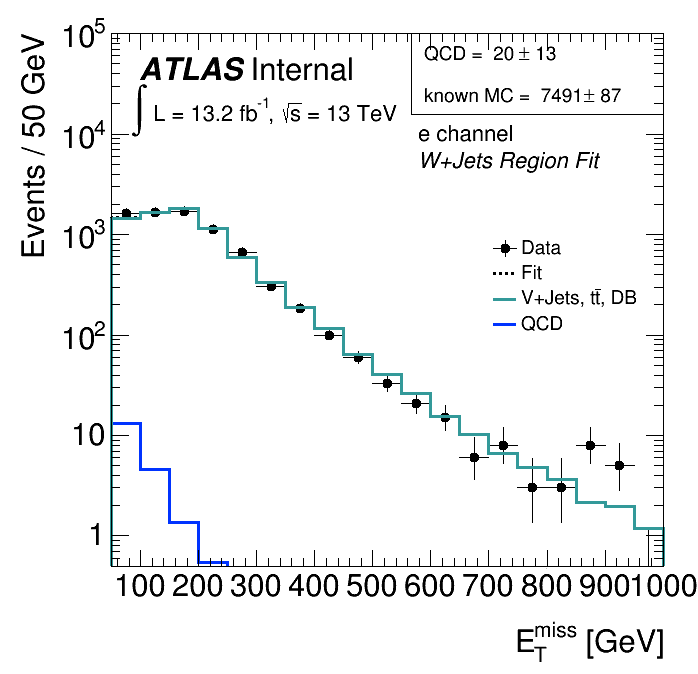
\includegraphics[width=.48\textwidth]{figures/Appendix/qcd/met_wjfit_el_lp}\label{fig:qcdshape_fit_el:d}}
\caption[Multijet estimation for the electron channel]{Multijet estimation for the $e$-channel. The shape extracted from the \protect\subref{fig:qcdshape_fit_el:a} high purity (HP) multijet region and \protect\subref{fig:qcdshape_fit_el:c} low purity (LP) multijet region is used to fit the \Wjets \protect\subref{fig:qcdshape_fit_el:b} HP CR and  \protect\subref{fig:qcdshape_fit_el:d} LP CR. Both fits show a negligible contamination for $\MET>100\,\GeV$.}
\label{fig:qcdshape_fit_el}
\end{figure}

\begin{figure}[htb]
\centering
\subfloat[]{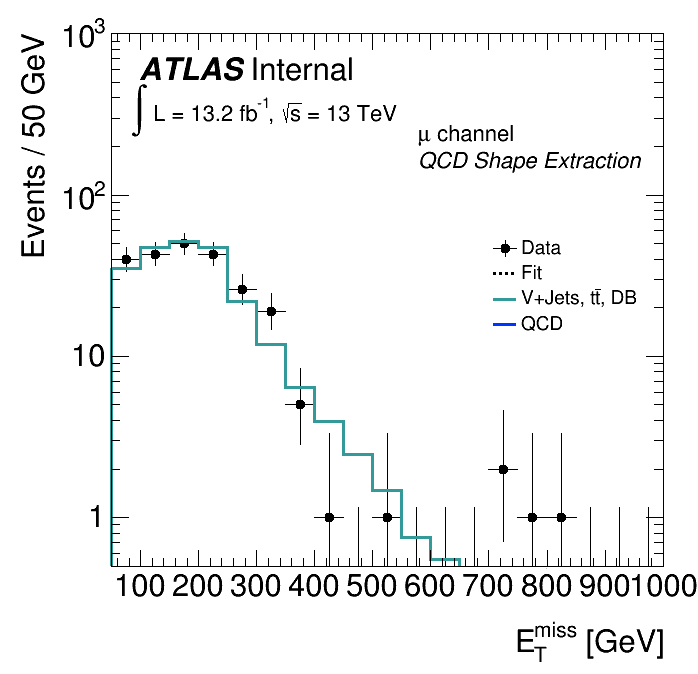
\includegraphics[width=.48\textwidth]{figures/Appendix/qcd/met_qcdshape_mu_hp}\label{fig:qcdshape_fit_mu:a}}
\subfloat[]{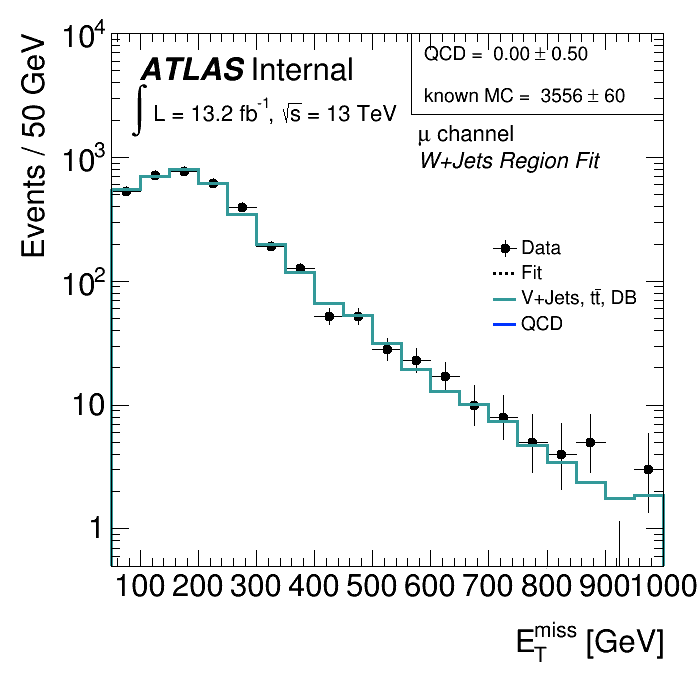
\includegraphics[width=.48\textwidth]{figures/Appendix/qcd/met_wjfit_mu_hp}\label{fig:qcdshape_fit_mu:b}}\\
\subfloat[]{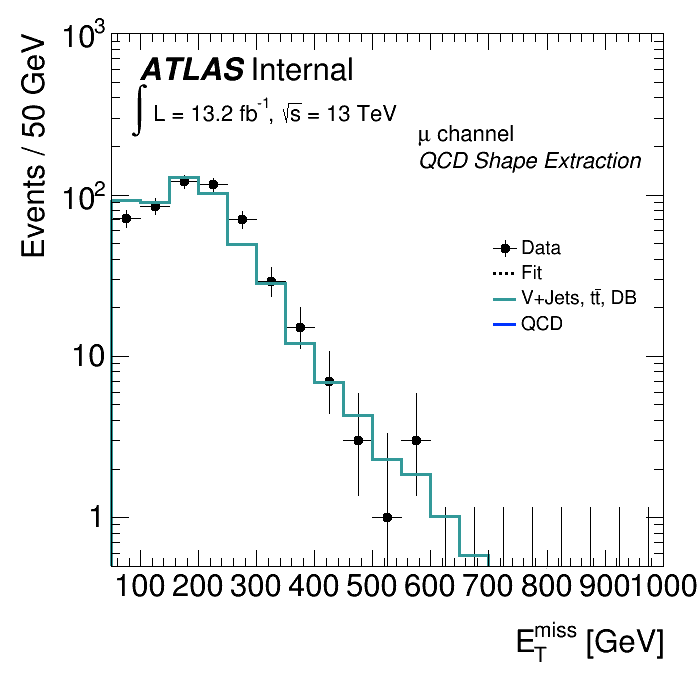
\includegraphics[width=.48\textwidth]{figures/Appendix/qcd/met_qcdshape_mu_lp}\label{fig:qcdshape_fit_mu:c}}
\subfloat[]{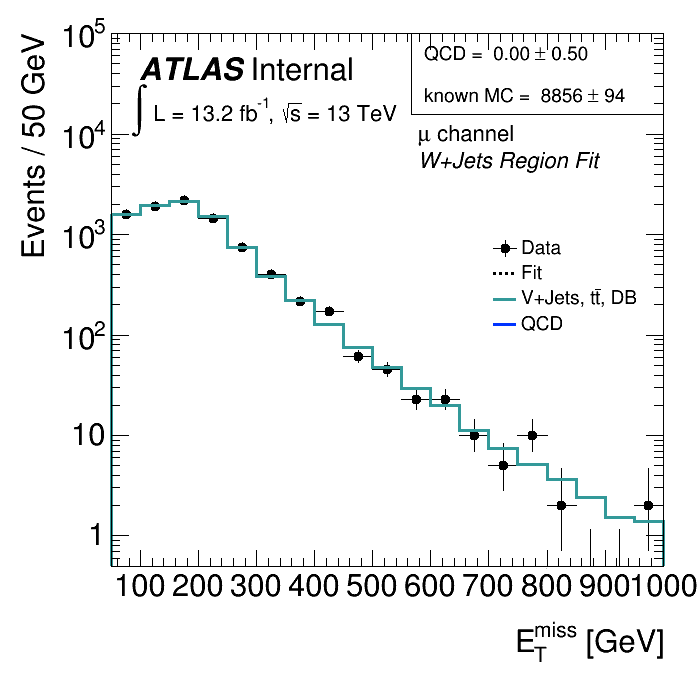
\includegraphics[width=.48\textwidth]{figures/Appendix/qcd/met_wjfit_mu_lp}\label{fig:qcdshape_fit_mu:d}}
\caption[Multijet estimation for the muon channel]{Multijet estimation for the $\mu$-channel. The shape extracted from the \protect\subref{fig:qcdshape_fit_mu:a} high purity (HP) multijet region and \protect\subref{fig:qcdshape_fit_mu:c} low purity (LP) multijet region shows a negligible multijet contribution. The fit in the \Wjets \protect\subref{fig:qcdshape_fit_mu:b} HP CR and \protect\subref{fig:qcdshape_fit_mu:d} LP CR is consistent with the MC simulated backgrounds.}
\label{fig:qcdshape_fit_mu}
\end{figure}	

\clearpage
A final check of the contamination in the high-$\pT(e)$ region is shown in ~\Fig{\ref{fig:qcdfit_highpt}}. The multijet contribution for $\MET>100\,\GeV$ is negligible. Thus, the multijet cut removes the mis-modeling in the high-\pT region for the $e$-channel, and the estimated QCD contamination in the signal regions and control regions is negligible. The multijet background is therefore neglected in this analysis.
\begin{figure}[tb]
\centering
\subfloat[]{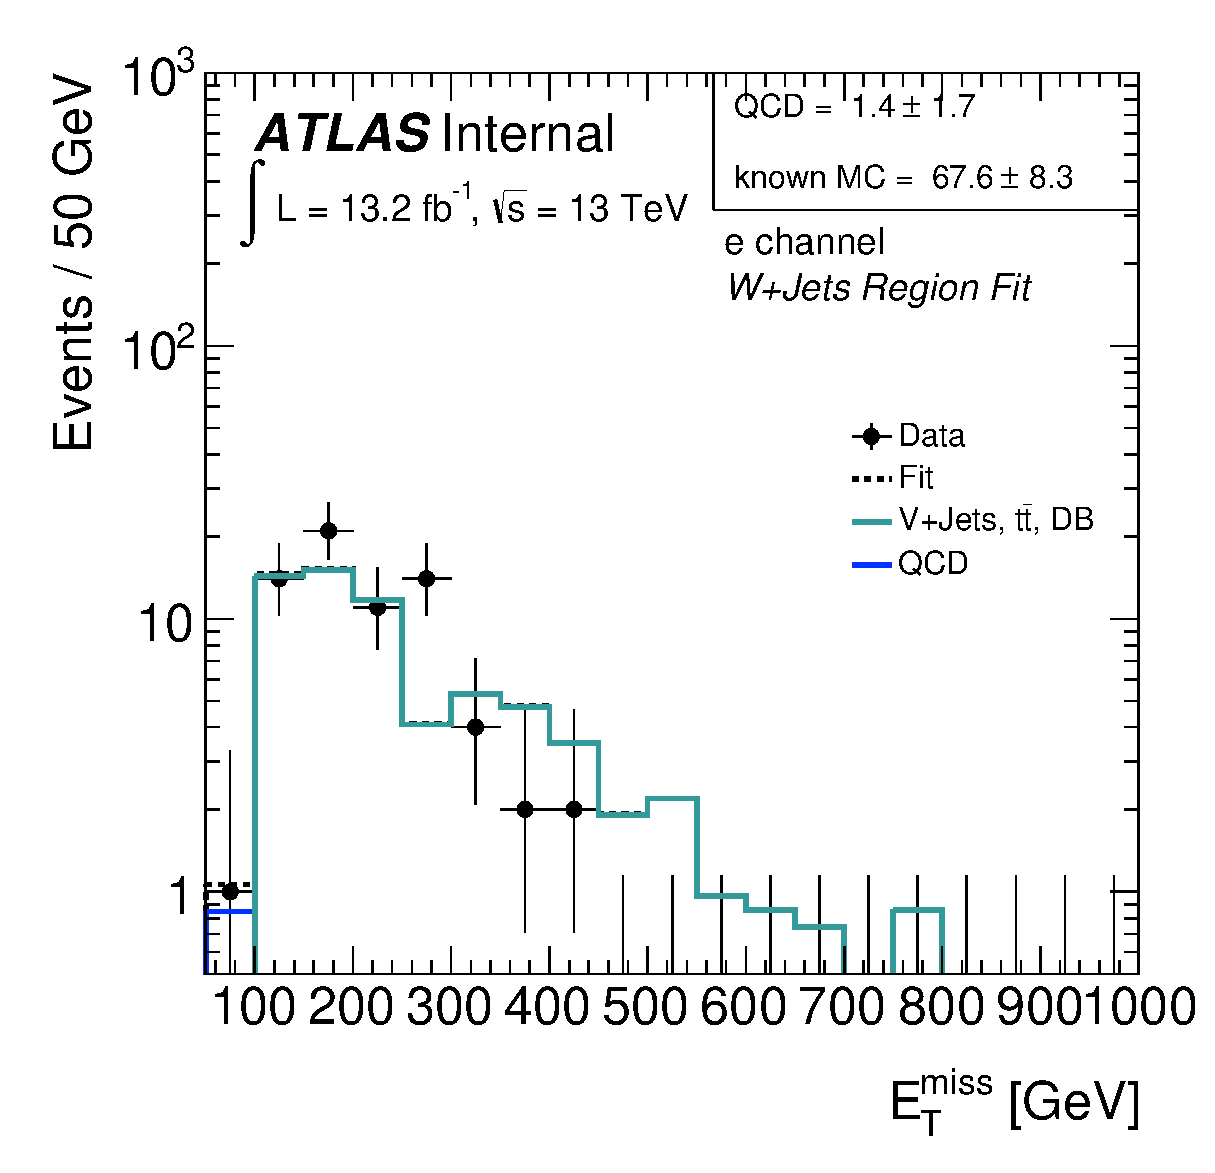
\includegraphics[width=.48\textwidth]{figures/Appendix/qcd/met_wjfit_el_hp_pt4}\label{fig:qcdfit_highpt:a}}
\subfloat[]{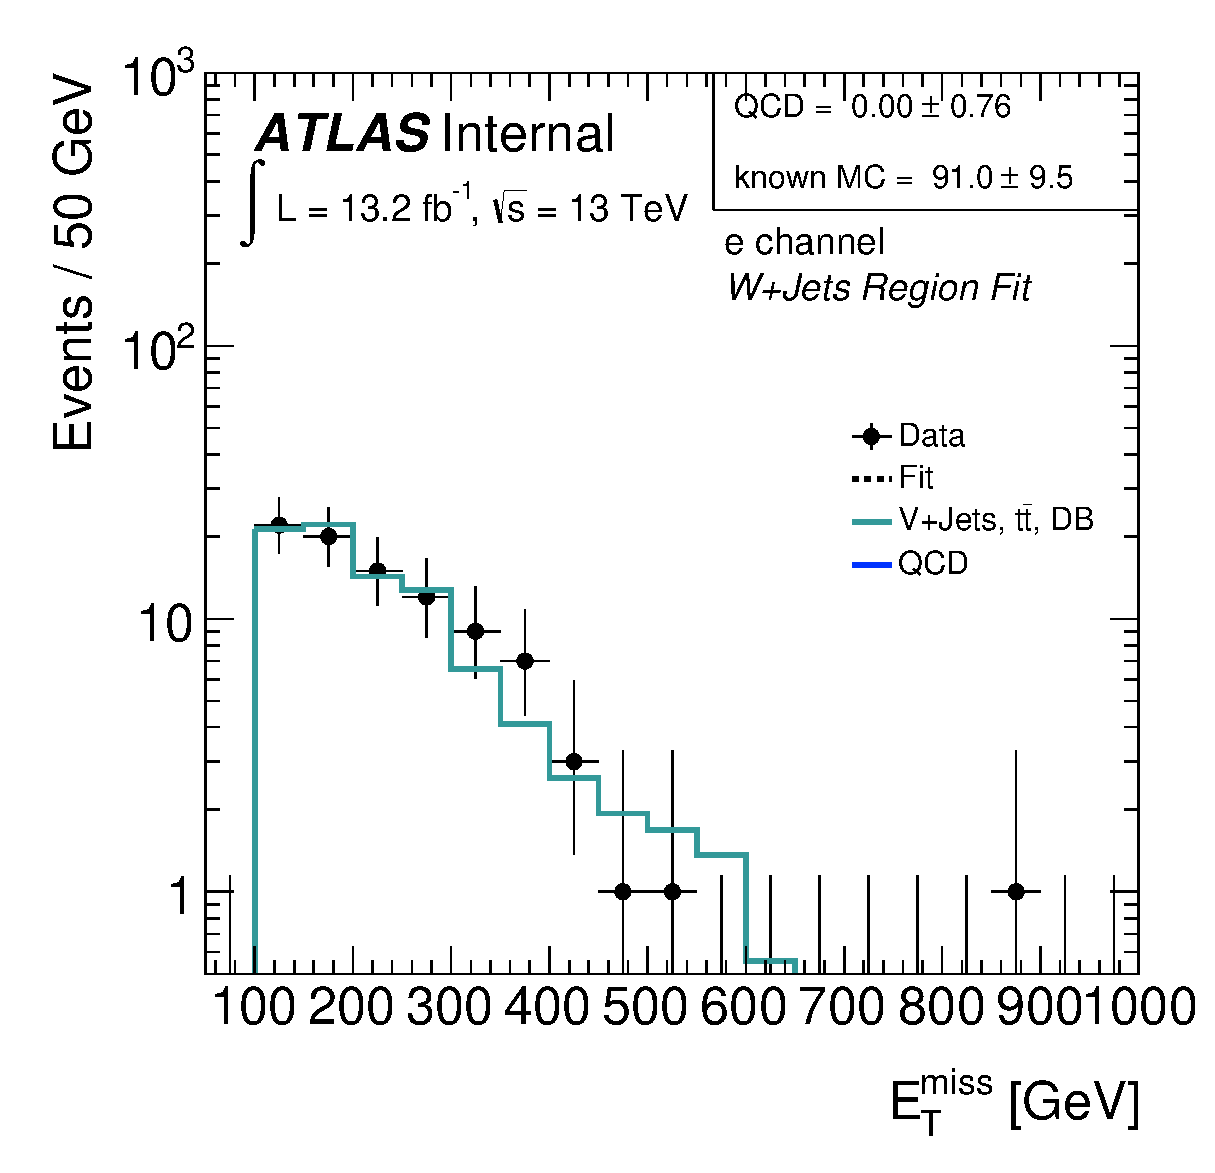
\includegraphics[width=.48\textwidth]{figures/Appendix/qcd/met_wjfit_el_lp_pt4}\label{fig:qcdfit_highpt:b}}
\caption[Multijet estimation for events with high transverse momentum electrons]{Multijet estimation in the $e$-channel for events with $\pT(e)>400\,\GeV$. The fit in the \Wjets \protect\subref{fig:qcdfit_highpt:a} high purity CR and \protect\subref{fig:qcdfit_highpt:b} low purity CR show a negligible contribution for $\MET>100\,\GeV$.}
\label{fig:qcdfit_highpt}
\end{figure}


